\documentclass{article}
\usepackage[utf8]{inputenc}
\usepackage[a4paper, margin=2.5cm]{geometry}
\usepackage{graphicx}
\usepackage[french]{babel}

\usepackage[default,scale=0.95]{opensans}
\usepackage[T1]{fontenc}
\usepackage{amssymb} %math
\usepackage{amsmath}
\usepackage{amsthm}
\usepackage{systeme}

\usepackage{hyperref}
\hypersetup{
    colorlinks=true,
    linkcolor=blue,
    filecolor=magenta,      
    urlcolor=cyan,
    pdftitle={SIGNAL},
    % pdfpagemode=FullScreen,
    }
\urlstyle{same} %\href{url}{Text}

\theoremstyle{plain}% default
\newtheorem{thm}{Théorème}[section]
\newtheorem{lem}[thm]{Lemme}
\newtheorem{prop}[thm]{Proposition}
\newtheorem*{cor}{Corollaire}
%\newtheorem*{KL}{Klein’s Lemma}

\theoremstyle{definition}
\newtheorem{defn}{Définition}[section]
\newtheorem{exmp}{Exemple}[section]
% \newtheorem{xca}[exmp]{Exercise}

\theoremstyle{remark}
\newtheorem*{rem}{Remarque}
\newtheorem*{note}{Note}
%\newtheorem{case}{Case}



\title{Traitement du signal}
\author{Charles Vin}
\date{2022}

\begin{document}
\maketitle

Cours de \begin{itemize}
    \item Hassam Aboushady, équipe CIAN : hassam.aboushady@lip6.fr. Cours inspiré des 5 premiers chapitre du livre "B.P.Lathi, Linear Signals \& Systems, Oxford University Press 2005" 
    \item Sebastien Baey : sebastien.baey@lip6.fr
\end{itemize}

Modalité d'examen : 
\begin{itemize}
    \item Un exam par professeur après chaque partie. 
    \item Pour Aboushady : 60\% exam, 40\% sur les CR de TD chaque semaine into 50\% de la note finale + une feuille A4
    \item Pour Baey à voir
\end{itemize}

Table des matières 
\begin{itemize}
    \item Signaux et opération utiles
    \item Traitement de signal dans le domaine Temporel (convolution) \begin{itemize}
        \item Temps continu
        \item Temps discret
    \end{itemize}
    \item Traitement de signal dans le domaine fréquentiel \begin{itemize}
        \item Transformé de Laplace (Temps continu)
        \item Transformé en Z (Temps discret)
    \end{itemize}
    \item Filtrage en temps continu/discret
\end{itemize}

Quatres type de signal : Temps continu/discret X Amplitude Analogique(continue)/numérique(discret). D'un point de vu technique, le type d'amplitude ne change pas grand chose (ça rajoute juste une erreur qu'on modélise comme du bruit). Ce qui est important est le type de temps.

\section{Opération sur les signaux}
\subsection{Quelques révisions}
On a \begin{itemize}
    \item Un signal $ x(t) $ en entrée
    \item Qui passe dans un système $ h(t) $ 
    \item Qui sort un autre signal $ y(t) $ 
\end{itemize}
3 opérations : Voir les graphique dans OneNote
\begin{itemize}
    \item Décalage : On décale le signal dans le temps $ x(t+T), x(t-T)$ 
    \item Etalage et compression dans le temps : \begin{itemize}
        \item Etalage : $ x(t/2) $ Aplatie la courbe dans le temps 
        \item Compression : $ x(2t) $ L'inverse
    \end{itemize}
    \item Inversion : $ x(-t) $ : symétrie par rapport à l'ordonnée. 
\end{itemize}

On vas écrire les fonctions de signal en utilisant cette fonction
\[
    \begin{cases}
        1 &\text{si } t \geq 0\\
        0 &\text{si } t > 0\\
    \end{cases} 
.\]
\begin{exmp}[]
    Exprimer $ x(t) $ en fonction de $ u(t) $. Voir OneNote
\end{exmp}

\begin{defn}[L'impulsion (dirac)]
    On mesure l'impulsion (le saut si on prend une porte) avec cette fonction. L'amplitude ici est infini ( mot du prof mais genre la pente est infini). 
    \[
        \delta (t) = 0 \text{ pour } t \neq 0 , \int_{- \infty }^{\infty } \delta (t) dt = 1
    .\]
    En faite il le mesure avec cette fonction mais il a fait un dessin où il fait tendre $ \epsilon \to 0 $ pour reserrer la fenêtre de l'intégrale autour de la porte 
\end{defn}

\begin{defn}[L'exponentiel]
    On passe dans les complexes où on écrit le nombre imaginaire avec $ i $ ou $ j $ (pour pas confondre le $ i $ de l'intensité du courant). \begin{align*}
        e^{st} \text{ avec } s &= a + jb \\
        e^{st} = e^{(a+jb)t} &= e^{at} e^{jbt} \\
                            &= e^{at}(\cos (bt) + j \sin bt)
    \end{align*}
\end{defn}

\subsection{La convolution}
\begin{defn}[]
    En gardant en tête la définition de tout à l'heure avec le signal d'entrée $ x(t) $ et le système $ h(t) $. On définie l'intégrale de la convolution tel que 
    \begin{align*}
        y(t) = x(t) \star h(x) &= \int_{-\infty}^{\infty } x(\tau  )h(t-\tau  ) d \tau  \\
        & = \int_{-\infty }^{\infty }h(\tau  )x(t-\tau    d \tau  )
    \end{align*}
\end{defn}
\begin{exmp}[]
    Déterminez la réponse d'un système définit par $ h(t) = e^{-2t} u(t)$  à une entrée $ x(t)=e^{-t}u(t) \to u(\tau ) $. 
    \begin{align*}
        y(t) = x(t) \star h(t) &= \int_{(\infty )}^{\infty } x(\tau )h(t-\tau )d \tau \\
        &= \int_{0}^{t}e^{-\tau }e^{-2(t-\tau )}d \tau 
    \end{align*}
    Voir figure \ref{exmp_conv_1}.
    \begin{figure}[!htbp]
        \centering
        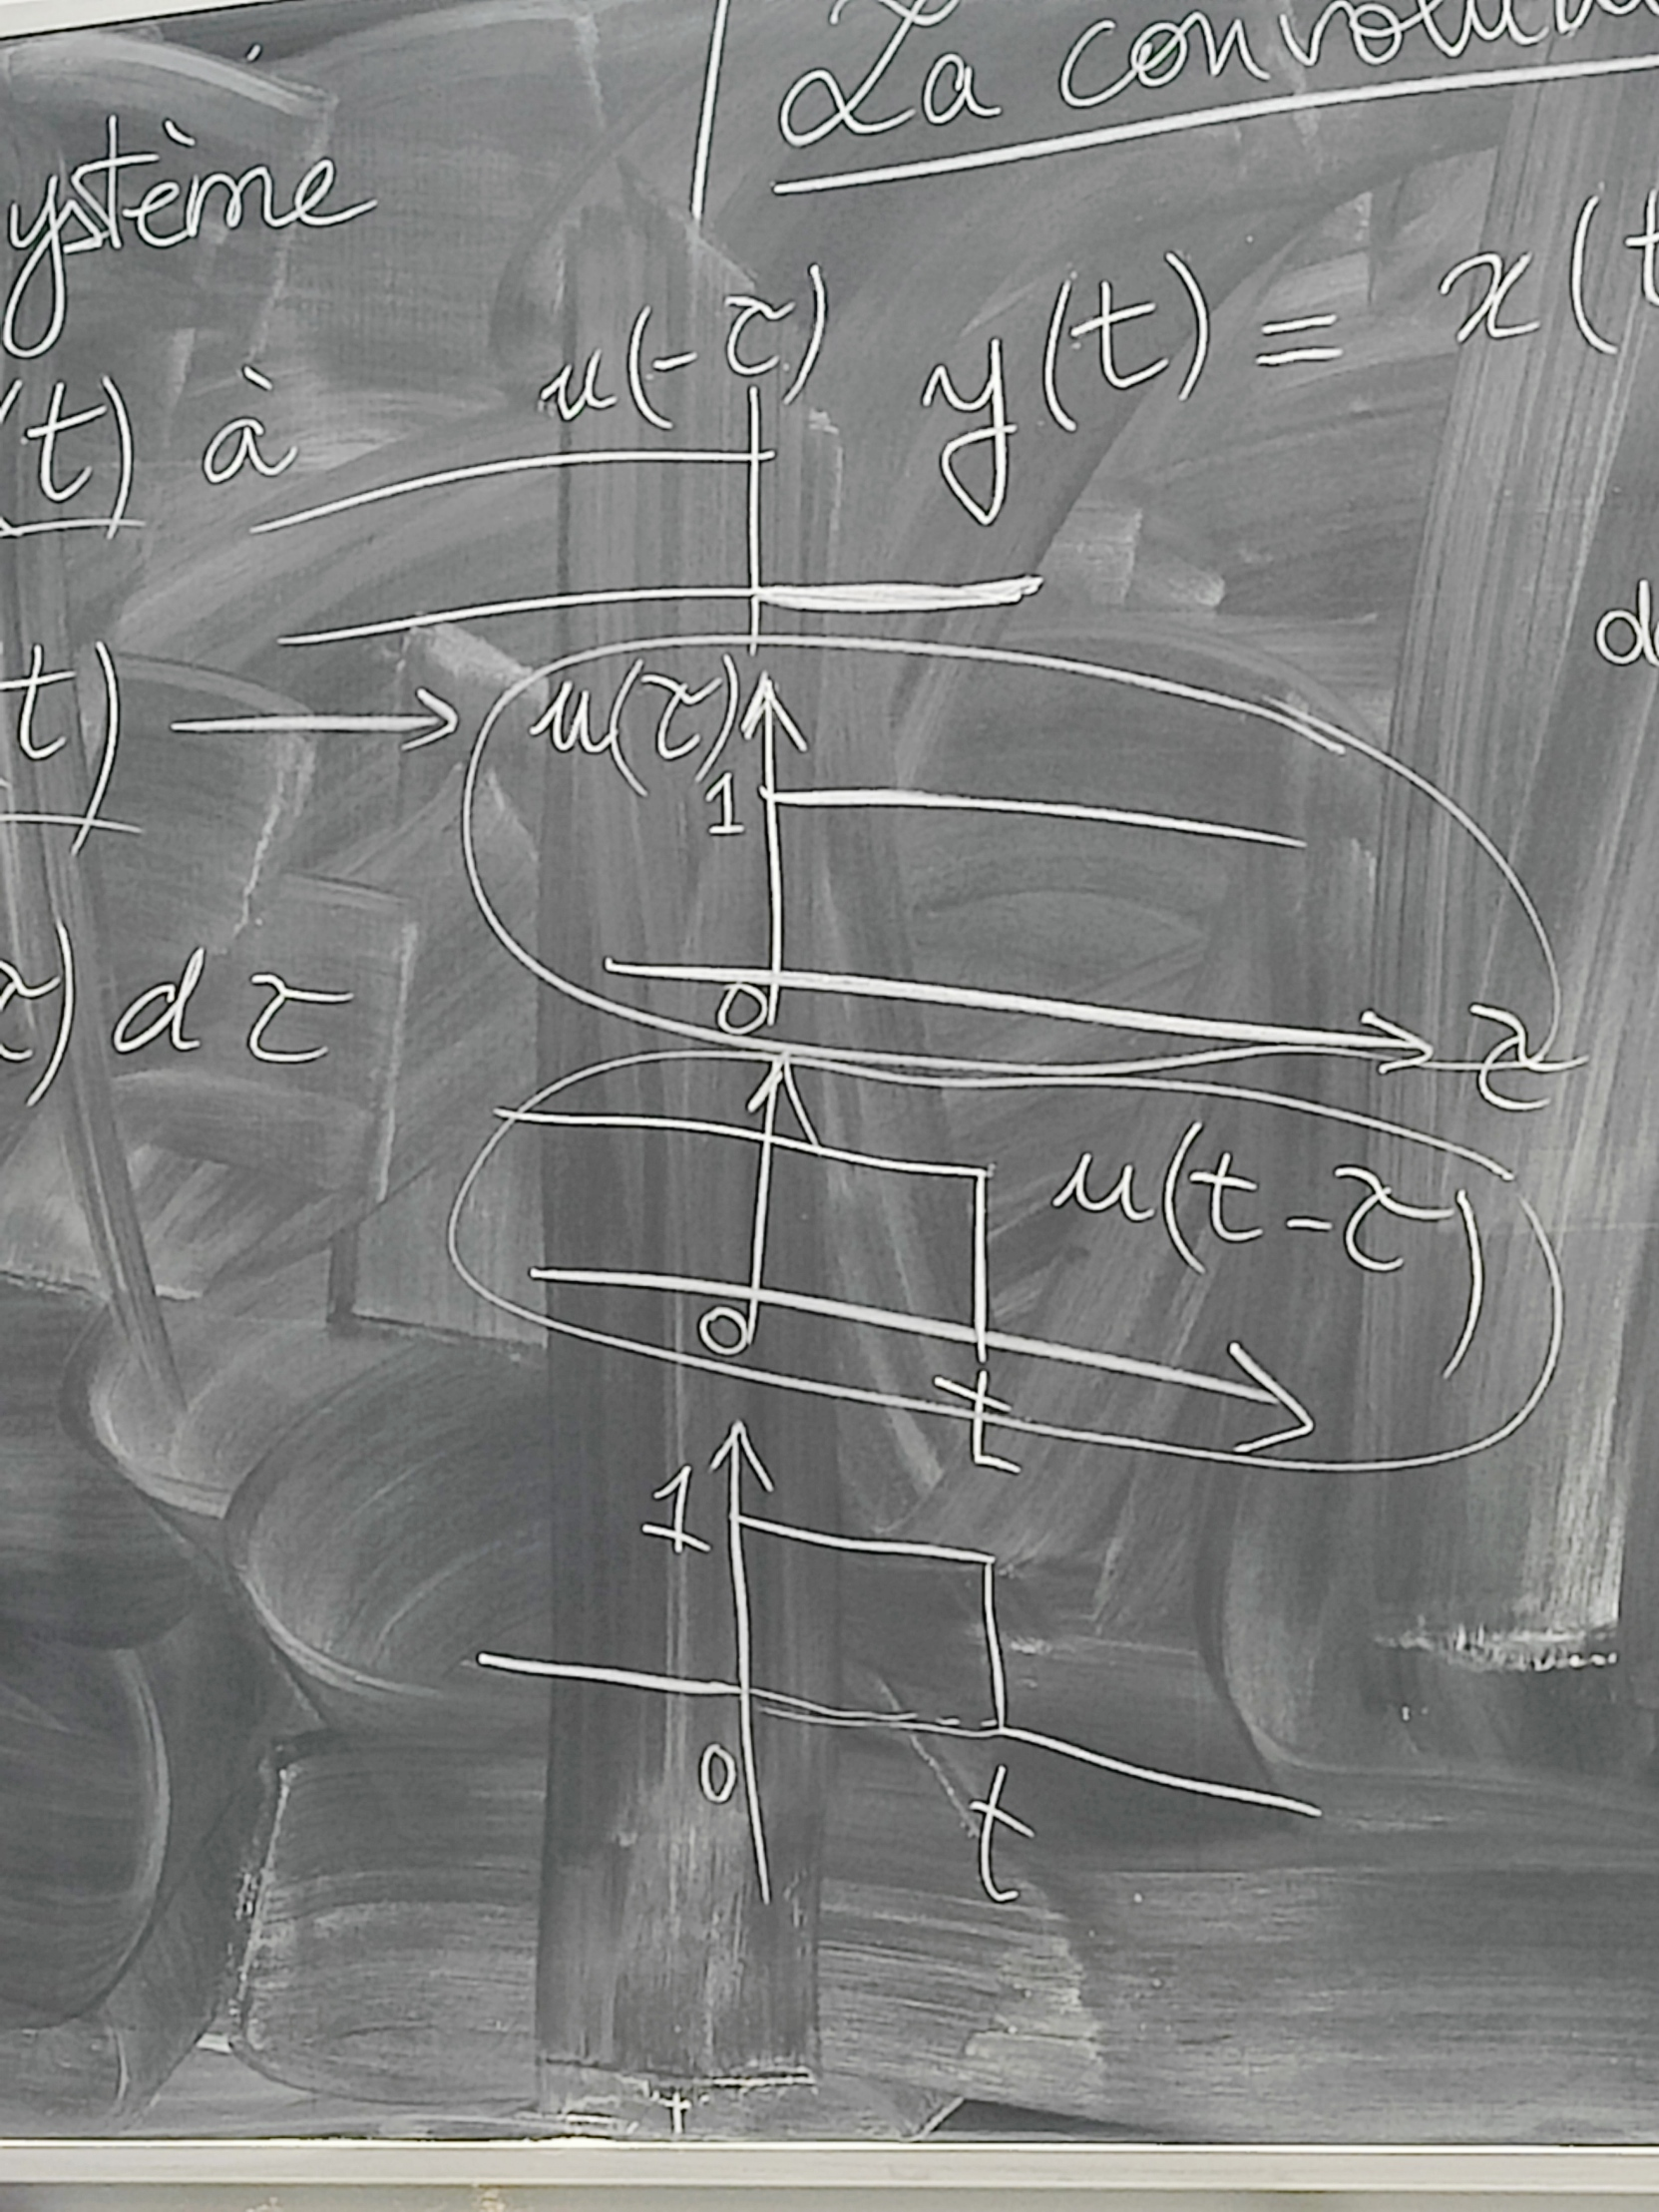
\includegraphics[width=.60\textwidth]{./figures/fig1.jpg}
        \caption{Exemple convolution}
        \label{exmp_conv_1}
    \end{figure}
\end{exmp}
\begin{prop}[de la convolution]
    Quelques propriété de la convolution
    \begin{itemize}
        \item Commutativité : $ x_1(t) \star x_2(t) = x_2(t) \star x_1(t) $ 
        \item Distributivité : toi même tu sais
        \item Associativité : $ x_1(t) \star x_2(t) \star x_3(t) = (x_1(t) \star x_2(t)) x_3(t) = x_1(t) \star (x_2(t) \star x_3(t)) $ 
        \item Décalage : Si $ x_1(t) \star x_2(t) = c(t) $ alors \begin{align*}
            x_1(t) &\star x_2(t-T) = c(t-T) \\
            x_1(t-T) &\star x_2(t) = c(t-T) \\
            x_1(t-T_1) &\star x_2(t-T_2) = c(t-T_1 - T_2) \\
        \end{align*}
        \item Convolution avec une impulsion : $ x(t) \star \delta (t) = x(t) $ 
        \item La durée de la convolution : On somme les deux durées (temps entre le zéro du début et celui de la fin). Soit un signal $ x_1(t) $ d'une durée $ T_1 $ et un signal $ x_2(t) $ d'une durée $ T_2 $. Alors $ x_1(t) \star x_2(t) $ à une durée de $ T_1 + T_2 $. 
    \end{itemize}
\end{prop}

\subsubsection{La convolution graphique de $ x(t) \star h(t) $ }
\begin{enumerate}
    \item Je garde $ x(\tau ) $ fixe (ou $ h(t) $ )
    \item Je trace $ h(-\tau ) $ (ou $ x(t) $ )
    \item Je décale $ h(-\tau ) $ pour une valeur de $ t $ (ou $ x(t) $ )
    \item J'intègre $ x(\tau )h(t -\tau ) $ dans chaque cas (ou inverses)
    \item Je répète 3. et 4. pour différentes valeurs de $ t $ 
\end{enumerate}
\begin{exmp}[]
    Trouvez la convolution de $ x(t), h(t) $. Voir one note
\end{exmp}



\end{document}